\section{Introduction to Common Metrics}\label{sect:metrics}
To evaluate the results achieved by \gls{ssd} (see \cref{sect:methodology}) and
make them comparable to diverging approaches, a set of metrics is introduced in
this section. While the central metric used in this paper is \nameref{subsect:mAP},
also \nameref{subsect:pixel-wise-metrics} are introduced.

\subsection{Pixel-wise Metrics}\label{subsect:pixel-wise-metrics}
As a prerequisite to \gls{map}, pixel-wise metrics such as \nameref{par:precision-recall},
\nameref{par:f-scores} and \nameref{par:iou} will be briefly explained in the
following.

\paragraph{Precision \& Recall}\label{par:precision-recall}
To the best of the author's knowledge, the most influential metric used in stamp 
detection is pixel-wise evaluation of the precision and recall
tuple~\cite{Nandedkar.2015b,Younas.2017,Ahmed.2013,Dey.2015,Micenkova.2011, Bhalgat.2016, Micenkova.2015,Nandedkar.2015b}.
Often, recall and precision are used in settings with class imbalance where they
provide a more sensible measure than accuracy. In the stamp detection, every
image pixel can be considered to be from one of two classes, either
\textit{stamp} (i.e.\ positive) or \textit{non-stamp} (i.e.\ negative). In
training and evaluation images, \textit{non-stamp}-pixels greatly outnumber
\textit{stamp}-pixels, thereby showing obvious class imbalance.

A definition of precision and recall is given in~\cite[423]{Goodfellow.2016} as
follows. Precision is the fraction of \glsdisp{tp}{\textit{true} positive (TP)}
pixels over all detected pixels (see \cref{eq:precision}). Recall is the fraction
of \glsdisp{tp}{\textit{true} positive} detections over all \gls{gt} pixels
(see \cref{eq:recall}). This relationship is visually depicted in \cref{fig:visual-precision-recall}.
\begin{align}
    \label{eq:precision}\text{Precision}    &= \frac{TP}{TP + FP}\\
    \label{eq:recall}\text{Recall}          &= \frac{TP}{TP + FN}
\end{align}
Intuitively, precision is the ``ability of a classifier to distinguish a
negative sample from [a] positive one''~\cite{Younas.2017}, while
recall is ``the ability of a classifier to classify all positive samples''~\cite{Younas.2017}.
\begin{figure}
    \centering
    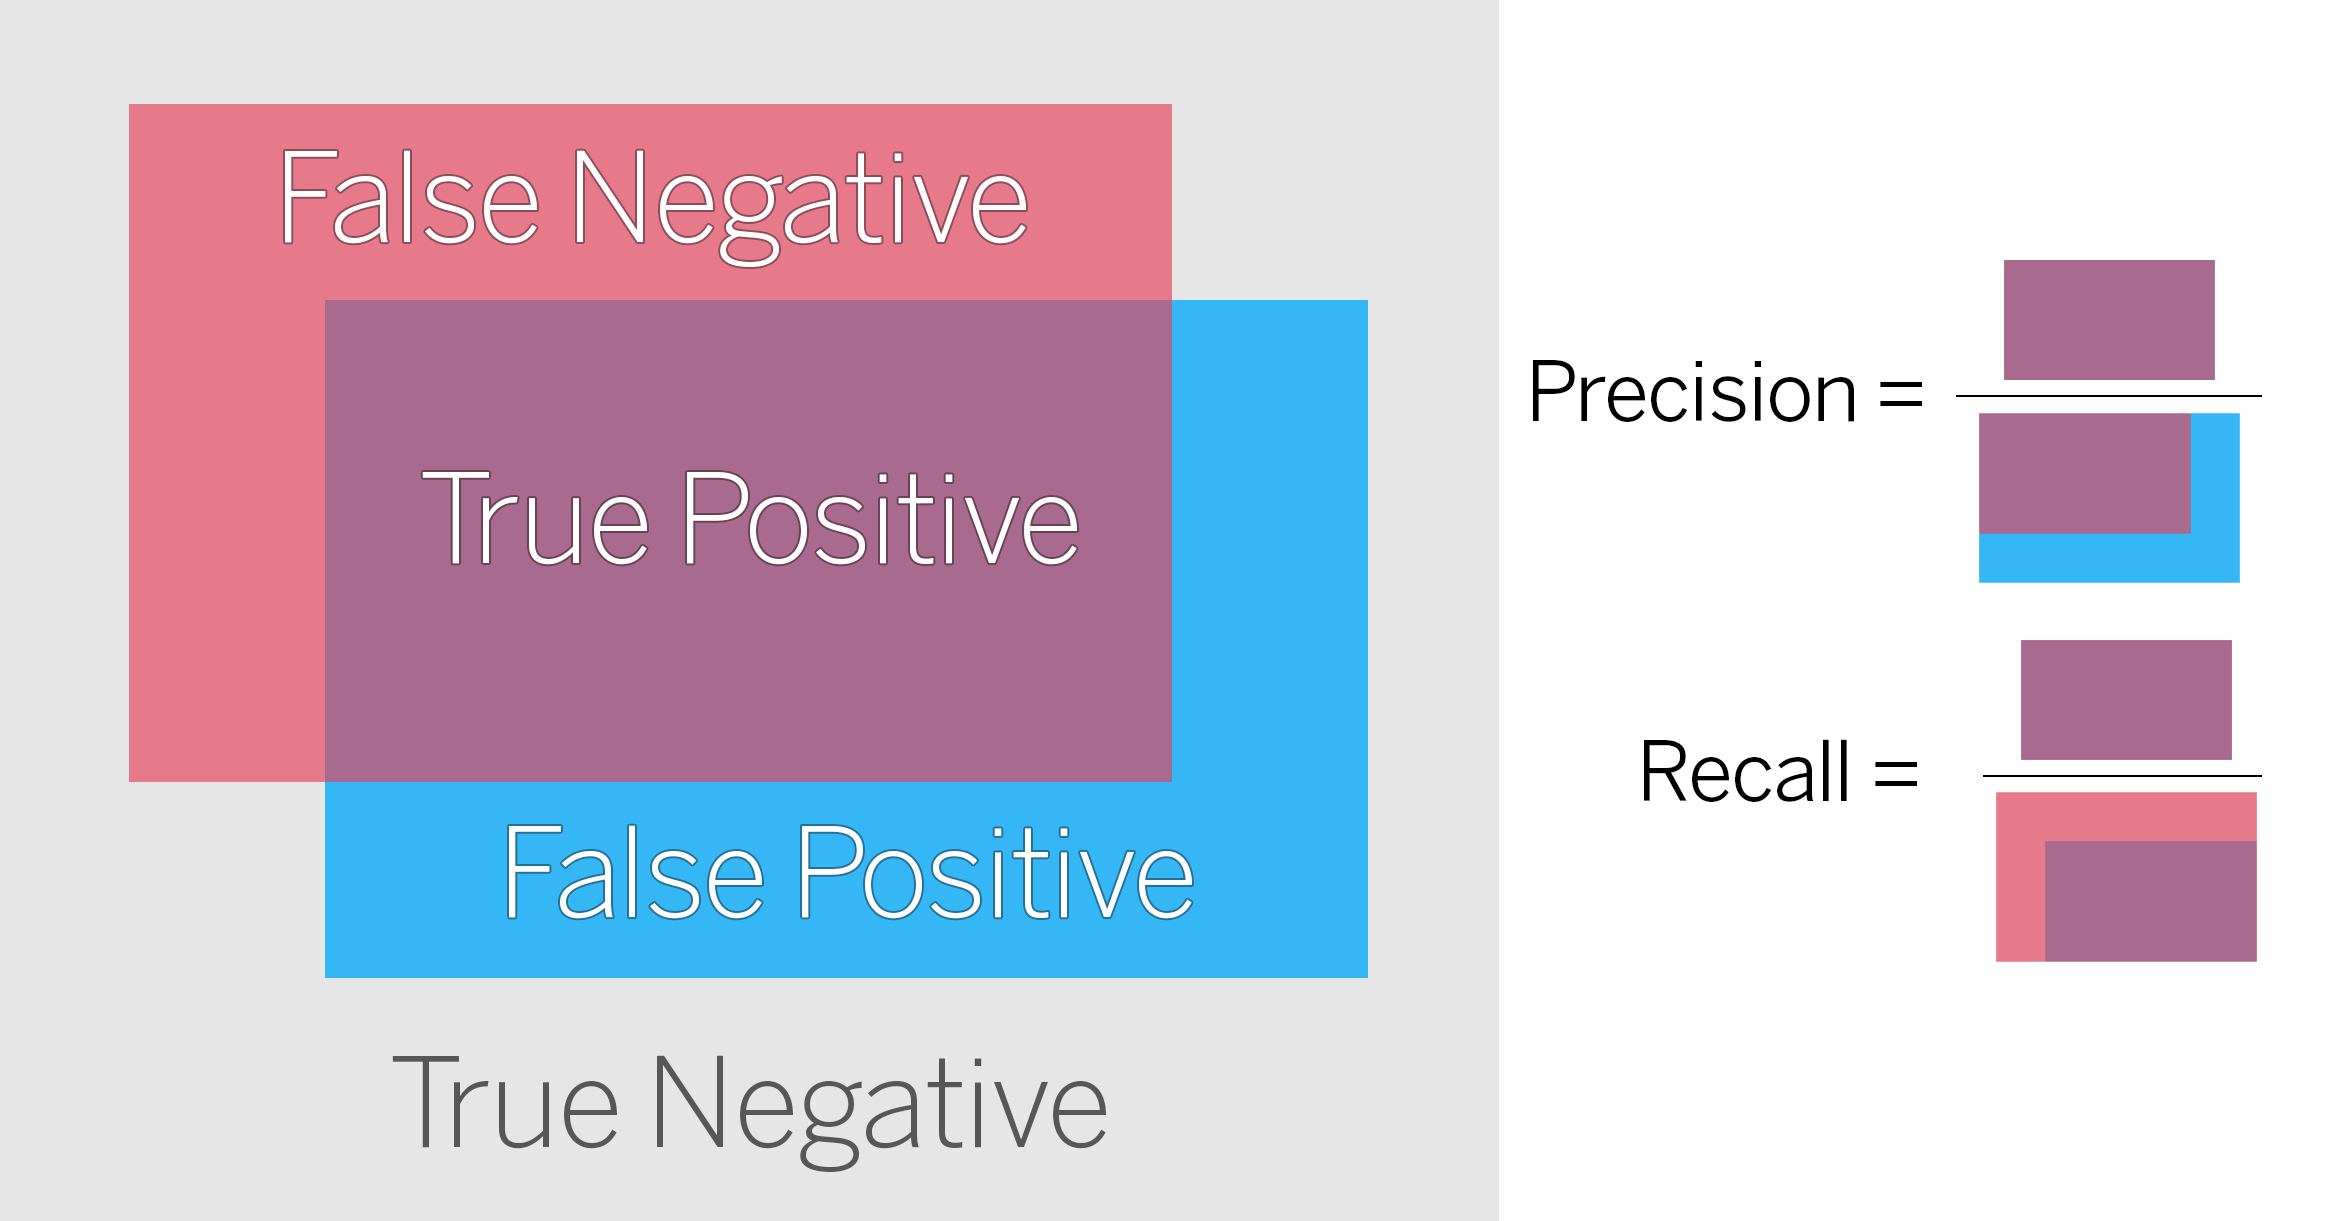
\includegraphics[width=.6\textwidth]{Metrics2.png}
    \caption[Visual example of pixel-wise recall, precision and \gls{iou}]
    {Visual example of pixel-wise recall, precision and \gls{iou}, with
    \gls{gt} (red) and detected pixels (blue)}\label{fig:visual-precision-recall}
\end{figure}

\paragraph{F-Scores}\label{par:f-scores}
Precision and recall can then be combined into a harmonic average, which is usually
called the family of \(F\)-Scores~\cite[e.g.][183]{Murphy.2012}. \(F_1\) is given
in~\cite[183]{Murphy.2012} as per \cref{eq:f1}.
\begin{equation}\label{eq:f1}
    F_1=\frac{2*\text{Precision}*\text{Recall}}{\text{Precision} + \text{Recall}}
\end{equation}
However, almost all works reviewed in \cref{sect:related-work} give only
precision \& recall and omit F-Scores.

\paragraph{Intersection over Union}\label{par:iou}
\Gls{iou}, also known as the Jaccard-Index or Jaccard-Similarity is a metric
closely related to \nameref{par:f-scores} via the Tversky-Index (for details on
this~\cite[cf.][Section 6.3 Similarity Measures]{James.2011}). \Gls{iou} is 
given by
\begin{equation}
    \text{IoU}=\frac{TP}{TP + FN + FP}
\end{equation}
Visually, this relation is shown also in \cref{fig:visual-precision-recall}.

\subsection{Class-wise Mean Average Precision}\label{subsect:mAP}
\Acrfull{map} is a widely used metric in object detection and was adopted by
well known tournaments such as \gls{coco}, \gls{voc}, and \gls{oi}. In context
of a multi-classification setting, \gls{map} represents the arithmetic mean
of \gls{ap} over the set of all classes. To understand \gls{map}, \acrshortpl{tp},
\acrshortpl{fp} \& \acrshortpl{fn} will be redefined for the object detection
setting in the following, then \gls{ap} will be explained.

\paragraph{TP, FP \& FN for Bounding Boxes}
Unlike in \fref{subsect:pixel-wise-metrics}, \acrshortpl{tp}, \acrshortpl{fp}
\& \acrshortpl{fn} are attributed not per individual pixel, but per \gls{bbox}.
A predicted box is considered \gls{tp}, if its (pixel-wise) \gls{iou} with a
\gls{gt} \gls{bbox} is greater than some threshold, \gls{fp} otherwise. This threshold
is often appended to the metric with an @-symbol.
A \gls{fn} is recorded when for a given \gls{gt} \gls{bbox} no prediction had an
overlap greater than the threshold.

For example, assume minimum \(\text{\gls{iou}}=0.5\)(@.50IOU). Then in
\cref{fig:bbox-precision-recall}, \glspl{bbox} \(A\) and \(B\) would be considered
\glspl{fp} due to their low \gls{iou}, while \gls{bbox} \(B\) is a \gls{tp}.
We count 1 \gls{tp}, 2 \gls{fp} and 1 \gls{fn} and thus observe
\(\text{Precision} = \frac{1}{3}, \text{Recall} = \frac{1}{2}\) (following
\cref{eq:precision,eq:recall}).

\begin{figure}[htp!]
    \centering
    \includegraphics[width=.3\textwidth]{metrics3.png}
    \caption[Visual example for bounding-box-wise confusion matrix]{Visual
    example for bounding-box-wise confusion matrix, with \gls{gt} \glspl{bbox}
    (red) and predicted \glspl{bbox} (blue). For each predicted \gls{bbox} a
    confidence score (percent) is given.}\label{fig:bbox-precision-recall}
\end{figure}

\paragraph{Precision-Recall-Curves and Average Precision}\label{par:precision-recall-curves-ap}
The Precision-Recall curve is constructed by first ordering the set of predicted
\glspl{bbox} for a class \mathvar{c} at a given threshold (e.g.\ 0.5\gls{iou})
by their confidence\footnotemark. Next, for every prediction in the ordered set
\(\mathbf{G}_c@.50\mathrm{IoU}\) determine whether it is a \gls{tp} or \gls{fp}. Finally,
step through \(\mathbf{G}_c@.50\mathrm{IoU}\), accumulate \glspl{tp} and \glspl{fp} and
report recall and precision for every element \(e_c\in \mathbf{G}_c@.50\mathrm{IoU}\),
and plot them. An example of this is shown in \cref{fig:precision-recall-curve}.

\footnotetext{A prediction has high confidence in the predicted class, if
\(\mathrm{confidence}=\max_{p\in \left[1, \abs*{C}\right]} \sigma(l_d^p)\) is high, e.g.\
\(\mathrm{confidence} \geq 0.9\) (excluding the \textit{no-object})}

\begin{figure}[htp!]
    \begin{subfigure}[t]{.49\linewidth}
        \centering
        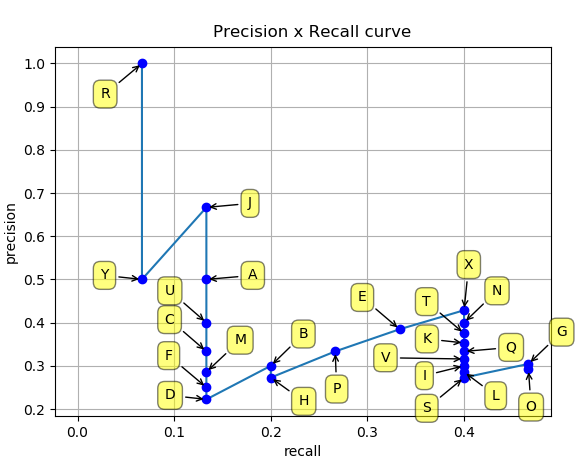
\includegraphics[width=.9\textwidth]{rafaelpadilla-precision-recall-curve.png}
        \subcaption{Precision-Recall-Curve. Each capital represents an inferred
        \gls{bbox}. Recall \& Precision are plotted by accumulating \gls{tp} and
        \gls{fp} over the list of inferred \glspl{bbox} sorted by confidence.}\label{fig:precision-recall-curve}
    \end{subfigure}
    \hfill
    \begin{subfigure}[t]{.49\linewidth}
        \centering
        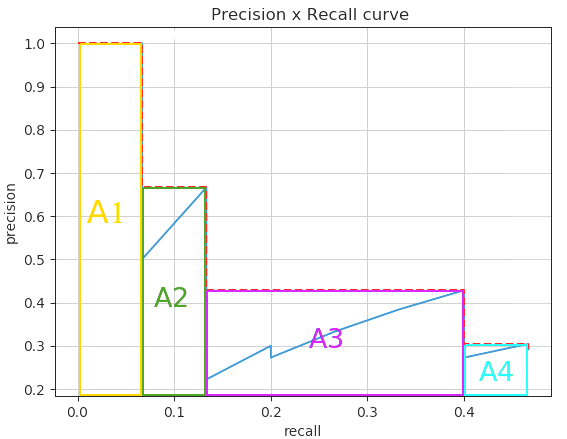
\includegraphics[width=.9\textwidth]{rafaelpadilla-average-precision.png}
        \subcaption{Interpolated Precision-Recall-Curve with drawn-in area under the
        curve, i.e.\ \gls{ap}.}\label{fig:interpolated-precision-recall-curve}
    \end{subfigure}
    \caption[Precision-Recall-Curve]{Precision-Recall-Curve and its
    interpolation. Both figures where adopted from~\cite{Padilla.2019}.}
\end{figure}

To improve comparability, the Precision-Recall-Curve \(f_c(r)\) for class \(c\)
can be smoothed by applying \(g_c(r) = \max (f(r), f(r')), \forall r' > r\), as
shown in \cref{fig:interpolated-precision-recall-curve}. The resulting curve is
then also called the \textit{Interpolated-Precision-Recall-Curve}. \gls{ap} is
now defined as the curve underneath the interpolated Precision-Recall-Curve
\(\operatorname{AP}_c = \int_{i=0}^{1} g_c(i) \,dx\).

Finally, \gls{map} is the mean of \gls{ap} over all classes \(C\). That is
\(\operatorname{mAP@.50IoU} = \frac{\sum_{c=1}^{\abs*{C}}\operatorname{AP}_c@.50\mathrm{IoU}}{\abs*{C}}\)
Despite its extensive use in the object detection community~\cite{Liu.2016,Ren.2015}, 
\gls{map} was only applied in a single work~\cite{Zhu.2006} from 2006. This is,
because 
\begin{enumerate*}[i.)]
    \item usually ranks are not generated in most approaches, therefore the 
    underlying metric of average precision, which \textit{is} computed over ranks, 
    lacks meaning and
    \item oftentimes stamp detection is framed as a binary classification problem.
\end{enumerate*}
\clearpage

\section{Additional illustrations for Section \fref{sect:results-and-discussion}}

\newcommand\cropim[1]{%
    %\ShellEscape{ubuntu run convert -trim figures/#1.png figures/#1-cropped.png}%
    #1-cropped.png
}

\begin{figure}[htp!]
    \begin{subfigure}[t]{.49\linewidth}
        \centering
        \includegraphics[width=.9\textwidth]{\cropim{samples/faint-stamp}}
        \subcaption{Faint Stamp}\label{fig:faint-stamp}
    \end{subfigure}
    \hfill
    \begin{subfigure}[t]{.49\linewidth}
        \centering
        \includegraphics[width=.9\textwidth]{\cropim{samples/multi-as-one}}
        \subcaption{Multiple stamps were detected as a single stamp}\label{fig:multi-as-one}    
    \end{subfigure}
    \\\bigskip{}
    \begin{subfigure}[t]{.49\linewidth}
        \centering
        \includegraphics[width=.9\textwidth]{\cropim{samples/logo-misdetection}}
        \subcaption{Logo detected as stamp}\label{fig:logo-as-stamp}    
    \end{subfigure}
    \hfill
    \begin{subfigure}[t]{.49\linewidth}
        \centering
        \includegraphics[width=.9\textwidth]{\cropim{samples/overlap-detected}}
        \subcaption{A stamp that was detected despite its overlap with text.}\label{fig:overlap-insample}
    \end{subfigure}
\end{figure}

\begin{figure}[htp!]
    \ContinuedFloat{}
    \centering
    \begin{subfigure}[t]{.49\linewidth}
        \centering
        \includegraphics[width=.9\textwidth]{\cropim{samples/bw1}}
        \subcaption{A black and white textual stamp.}\label{fig:black-and-white}
    \end{subfigure}
    \caption{Examplary results}
\end{figure}

\begin{figure}[htp!]
    \begin{subfigure}[t]{.49\linewidth}
        \centering
        \includegraphics[width=.8\textwidth]{\cropim{samples/out-of-sample-stamp}}
        \subcaption{A stamp from a different distribution}\label{fig:different-stamp}
    \end{subfigure}
    \hfill
    \begin{subfigure}[t]{.49\linewidth}
        \centering
        \includegraphics[width=.8\textwidth]{\cropim{samples/out-of-sample-overlap}}
        \subcaption{Although the stamp is extracted from \gls{staver}, it was placed
        in a different document by the author. Also see the significant overlap.}\label{fig:diff-domain-overlap}    
    \end{subfigure}
\end{figure}

\begin{figure}[htp!]
    \ContinuedFloat{}
    \centering
    \begin{subfigure}[t]{\linewidth}
        \centering
        \includegraphics[width=.95\textwidth]{\cropim{samples/many}}
        \subcaption{An example with many stamps in one image.}\label{fig:many-in-one}    
    \end{subfigure}
    \\\bigskip{}
    \begin{subfigure}[t]{\linewidth}
        \centering
        \includegraphics[width=.95\textwidth]{\cropim{samples/wiki1}}
        \subcaption{A difficult different distribution.}\label{fig:difficult-diff-domain}    
    \end{subfigure}
    \caption{Examples from different domains}\label{fig-diff-domains}
\end{figure}